This chapter addresses the hardware architecture. It starts by setting up \textit{VexRiscv}, \textit{Versat} and \textit{Timer} in the IOb-MP2-E. Then, it describes two hardware accelerators that were developed to accelerate the \textit{psycho\_3\_threshold} function. In the end, a system overview is done.

In the initial stage of this work, the IOb-MP2-E system comprised eight main components: \textbf{AXI}, an AXI interconnect protocol;
\textbf{CACHE}, a high-performance Verilog cache; \textbf{LIB}, a set of \textit{Verilog} macros; \textbf{MEM}, a set of memory Verilog descriptions; \textbf{PICORV32}, a RISC-V processor; \textbf{TWOLAME}, an optimized MP2 encoding software; \textbf{UART}, a UART core; \textbf{DDR4 Controller}, a controller for DDR memory (figure~\ref{fig:newiob1}).
As previously stated, the ultimate goal of this work is to develop a system that beats the only MPEG1/2 Layer II encoding IP core on the market, the \textit{CWda74}~\cite{CWda74}. This system uses fixed-point precision, and so the most logical approach to the problem turns out to be implementing the \textit{TwoLAME} algorithm using floating-point precision.  
Looking at the \textbf{PICORV32} CPU available, porting the software in these conditions would be undoable, due to its fixed-point arithmetic limitation.

\subsection{VexRiscv}

For this reason, the current CPU has to be substituted, and the \textbf{VEXRISCV} becomes the premier pick, as it includes a floating-point unit (FPU)~\cite{fpu}. In this process, the \textit{PICORV32} was removed from the IOb-MP2-E and the \textit{VEXRISCV} was added as the only CPU (figure~\ref{fig:newiob1}). This was straightforward, as \textit{VEXRISCV} was previously implemented and tested by \textit{IObundle, Lda}. Apart from adding the submodule to IOb-MP2-E's repository, some paths were changed to allow the correct compilation of the CPU. Interrupt signals were also added to the system data bus, such as \textit{timerInterrupt}, \textit{softwareInterrupt}, and \textit{externalInterrupt}. 
%explain vexriscv

%In the context of hardware acceleration, it is crucial to understand the hardware architecture of IOb-MP2-E, especially its synthesis and FPGA implementation. Therefore, a description of how the software integrates with the hardware is presented below.

\subsection{Versat}

Given \textit{Versat} being the optimal choice for accelerating \textit{TwoLAME} algorithm, integration into IOb-MP2-E becomes imperative.
Therefore, the first step in this process was adding \textbf{VERSAT} to the IOb-MP2-E (figure~\ref{fig:newiob1}). This was simple as \textit{VERSAT} was previously implemented and tested by \textit{IObundle, Lda}. Apart from adding it as a submodule to IOb-MP2-E's repository, some paths were changed to allow correct compilation.
The second step was more complex, consisting of adding an AXI interconnection between \textit{Versat} and IOB-MP2-E's external memory (DDR4 SDRAM). The system usually contains a single AXI~\cite{bib:axi_xilinx} interconnect instance, used by external memory and CPU. Therefore, a pragmatic solution was to double the wire size of the existing AXI interconnection, providing communication from/to \textit{Versat} while keeping the same AXI instance.

\subsubsection{Functionality and Interfaces}

Focusing on the \textit{Versat} matter, \textit{versatSpec.txt} functions like a code script, while \textit{Versat} operates akin to a compiler. In other words, \textit{Versat} takes the code, described in a Domain Specific Language (DSL), and generates not only the accelerator (in Verilog) but also the necessary headers and C source code. The generated code empowers the firmware to govern the accelerator effectively, i.e. it ensures correct correspondence between CPU actions and the accelerator.

\textit{Versat} generates hardware accelerators according to the dataflow paradigm. The algorithm is implemented by instantiating functional units (specified in \textit{versatSpec.txt}) and connecting them to execute the intended part of the algorithm. \textit{Versat} handles data validity transparently from the user, inserting buffer units between connections to ensure data from convergent paths arrive at the same time when needed.
Regarding the accelerator's internal registers, some of these registers are constant and shared by all accelerators, such as Direct Memory Access (DMA) and control registers. On the opposite, others depend on the specific functional units present in the accelerator.
The FUs need to implement certain interfaces recognizable by \textit{Versat} in order to perform useful work. Most FUs implement input and output ports in order to connect with other FUs. \textit{Versat} gives one the possibility to create and add new Functional units to the source. Furthermore, FUs can implement a variety of interfaces that allows them to receive or send data to outside the accelerator:

\begin{itemize}
    \item \textbf{Configuration:} Inputs that allow the CPU to modify and control the functionality of individual units. A configuration register connects to the configuration entries of each unit, conditioning its behavior. 
    \item \textbf{State:} Outputs that allow the CPU to read data from the units. Useful for small amounts of data transfer.
    \item \textbf{Memory-Mapped:} Allocation of specific address space for units, allowing access to them through read and write operations. This interface is primarily used for memory units, enabling the CPU to read and write data as required.
\end{itemize}

The accelerator generated by \textit{Versat} groups all these interfaces into a single memory-mapped interface, accessed by the CPU. When the CPU accesses an address inside the accelerator memory space, the CPU can be accessing a control register of the accelerator, the configuration, or the state registers (which are connected to the configuration and state interfaces of their specific units) or it can be accessing the FUs directly through the memory mapped interface.
Moreover, a DMA mechanism is used for efficient data transfers between the accelerator and external memory, specifically between the accelerator's memory-mapped interfaces and DDR. This DMA is configured by the CPU. In practice, the accelerator loads memories such as \textit{LTtm}, \textit{LTnm}, \textit{freq\_subt}, and $mem\to dbtable$ using the DMA, enabling efficient and high-speed data movement.

\subsection{Timer}
To allow profiling the \textit{TwoLAME} algorithm, another component was added to IOb-MP2-E, the \textbf{TIMER}~\cite{bib:iobtimer}. This peripheral is a 64-bit hardware timer, equipped with reset, enable, and reading functions. It includes a software driver and an example C application, which helps understand how it works. 
Similarly to the other components, the TIMER is tracked by a \textit{GitHub} repository (forked from \textit{IObundle, Lda}), integrating the IOb-MP2-E as a submodule. This component was previously implemented and tested by \textit{IObundle, Lda} as well. In addition, some paths were added to allow correct compilation. 
Figure \ref{fig:newiob1} shows a high-level block diagram of the IOb-MP2-E system at this point.

\vspace{0.1cm}

\begin{figure}[H]
\centerline{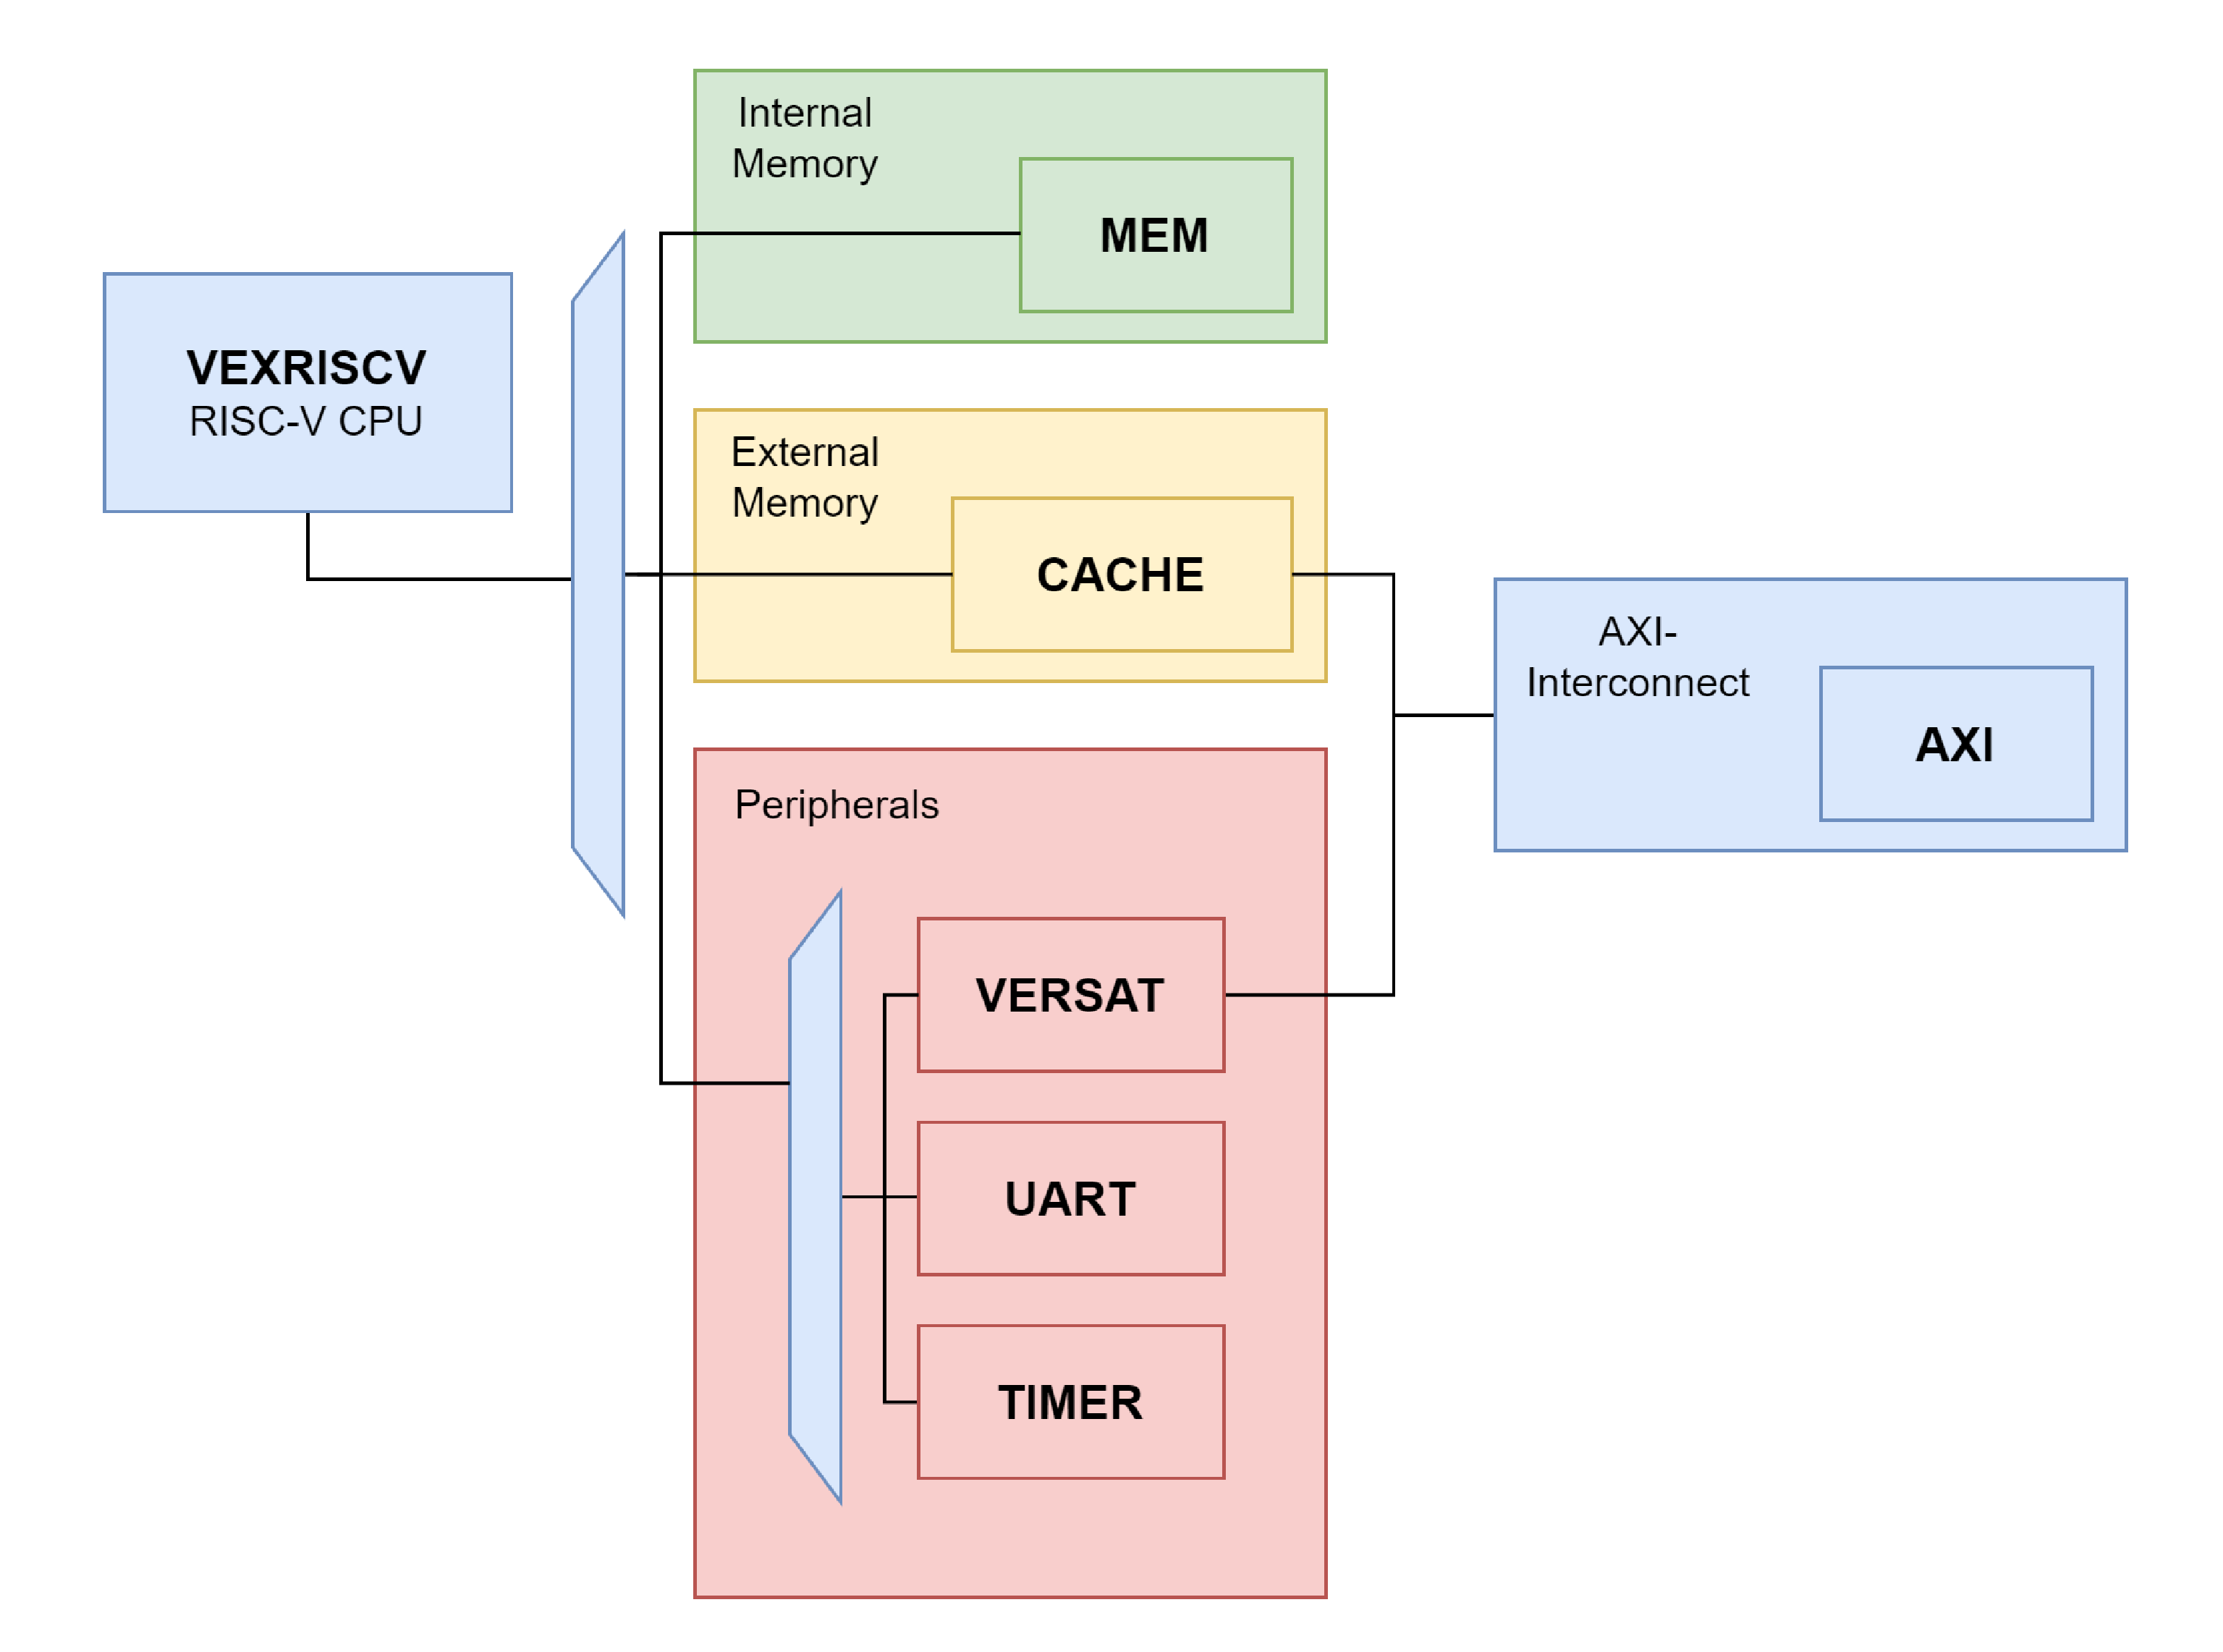
\includegraphics[width=0.85\linewidth]{iob2.pdf}}
\caption{High-level block diagram of the IOb-MP2-E in use.}
\label{fig:newiob1}
\end{figure}

\vspace{0.1cm}

Based on the results of \textit{TwoLAME}'s profiling, shown in \textit{Results} section, the subsequent step involves developing the hardware accelerators for the \textit{psycho\_3\_threshold} function, using \textit{Versat}.
The \textit{psycho\_3\_threshold} function contains three for loops, with the first one being a simple initialization process, setting each element of arrays \textit{LTtm} and \textit{LTnm} to a constant value (\textit{DBMIN}) within the range of 0 to 135 ($SUBSIZE-1$). Performing this initialization in hardware incurs unnecessary overhead, as the result remains constant for all iterations. Instead, in a hardware implementation, we can directly use the constant value DBMIN as an input for the subsequent hardware operations (the next for loops, in this case), optimizing efficiency and reducing the need for a dedicated initialization loop.
Therefore, only two accelerators should be developed to execute the second and third for loops of \textit{psycho\_3\_threshold}.
The third for loop is simple as it just includes the \textit{psycho\_3\_add\_db} function. 
On the opposite, the second for loop is not only complex but it is also more interesting. The main for loop (outer loop) contains two \textit{if} conditions and, inside each condition, there is another for loop (inner loop). Moreover, the inner loop is the same in both conditions, differing only on part of the input data. This means that it is only necessary to develop hardware that executes both inner loops, with the if conditions and the outer loop being handled by the CPU.

Before developing the accelerators, it is crucial to determine the control and data paths of the loops that are intended to be accelerated. In other words, the paths refer to the fundamental components that dictate how the software interacts with the hardware to achieve acceleration.
The control path defines the flow and sequencing of operations within the software that need to be accelerated. It includes decisions, branching, loops, and other control structures that determine the program's behavior~\cite{datacontrolpath}. Determining the control path is vital for optimizing the hardware design to efficiently execute these operations.
The data path refers to the route through which data flows within the software during its execution. It involves operations and transformations applied to the input data to produce the desired output. Understanding the data path is crucial for designing hardware components that can process and manipulate the data effectively to accelerate the software's performance.

\subsection{\textit{spectrum\_search} accelerator}

\subsubsection{Control and Data paths}
This section shows both control and data paths of the first accelerator, \textit{spectrum\_search}, corresponding to the second for loop in the original \textit{psycho\_3\_threshold} function.

\begin{figure}[H]
\centerline{\fbox{\includegraphics[width=0.90\linewidth]{first.pdf}}}
\caption{Control and data paths of the \textit{spectrum\_search} hardware accelerator.}
\label{data1}
\end{figure}

\subsubsection{Functional units}
Based on the previous Control and Data path, five FUs were designed to allow developing the \textit{spectrum\_search} accelerator (and also \textit{masking\_threshold}), such as \textit{FloatLess}, \textit{FloatGreater}, \\ \textit{FloatGreaterEqual}, \textit{Mux4} and \textit{Conditional1}.

A brief description of each functional unit is provided in the table below.

\vspace{0.5cm}

\begin{table}[H]
    \centering
    \begin{tabular}{|c|p{0.7\linewidth}|}
        \hline
        \multicolumn{1}{|c|}{\textbf{FU}} & \multicolumn{1}{c|}{\textbf{Description}} \\
        \hline
        \multirow{6}{*}{\textit{FloatLess}} & This module receives two 32-bit floating-point inputs and outputs a 32-bit value (repeated 1-bit result 32 times) indicating whether the first input is less than the second. It performs a comparison operation to determine if the first input is less than the second. If the first input is less than the second, the output will be a 32-bit value with all bits set to 1; otherwise, the output will be a 32-bit value with all bits set to 0.  \\
        \hline
        \multirow{6}{*}{\textit{FloatGreater}} & This module receives two 32-bit floating-point inputs and outputs a 32-bit value (repeated 1-bit result 32 times) indicating whether the first input is greater than the second. It performs a comparison operation to determine if the first input is greater than the second. If the first input is greater than the second, the output will be a 32-bit value with all bits set to 1; otherwise, the output will be a 32-bit value with all bits set to 0. \\
        \hline
        \multirow{6}{*}{\textit{FloatGreaterEqual}} & This module receives two 32-bit floating-point inputs and outputs a 32-bit value (repeated 1-bit result 32 times) indicating whether the first input is greater than or equal to the second. It performs a comparison operation to determine if the first input is greater than or equal to the second. If the first input is greater than or equal to the second, the output will be a 32-bit value with all bits set to 1; otherwise, the output will be a 32-bit value with all bits set to 0. \\
        \hline
        \multirow{5}{*}{\textit{Mux4}} & This module receives four 32-bit inputs and one 32-bit control input. It operates as a 4-to-1 multiplexer, selecting one of the 32-bit inputs based on the two least significant bits (LSB) of the control input.  The two LSB of the control input can be '00', '01', '10', or '11', selecting the first, the second, the third, or the fourth input, respectively. The output will be the 32-bit input that was selected. \\
        \hline
        \multirow{4}{*}{\textit{Conditional1}} & This module receives two 32-bit inputs and one 32-bit control input. It operates as a 2-to-1 multiplexer, selecting one of the 32-bit inputs based on the 32-bit control input. If the LSB of the control input is zero, the output will be the second 32-bit input; otherwise, the output will be the first 32-bit input. \\
        \hline
    \end{tabular}
    \caption{New \textit{Versat} functional units.}
    \label{tab:fu}
\end{table}

\vspace{0.5cm}

\subsubsection{Modules}
After analyzing the control and data paths, the hardware accelerator is developed in \textit{versatSpec.txt}. This file specifies the whole data process, which can be divided into several modules each representing a certain functionality or output. The starting module is called \textit{start} and invokes all the other modules.

A brief description of each module is provided in the list below.

\vspace{0.5cm}

\textit{\textbf{av}}

\begin{enumerate}

\item Float multiplication (\textit{mul1}):
\begin{itemize}
\item Takes \textit{const2} and \textit{bark} as inputs.
\item Multiplies \textit{const2} and \textit{bark}.
\end{itemize}

\item Float addition (\textit{add1}):
\begin{itemize}
\item Takes the output of \textit{mul1} and \textit{const1} as inputs.
\item Adds \textit{mul1} and \textit{const1}.
\end{itemize}

\item Float addition (\textit{add2}):
\begin{itemize}
\item Takes the output of \textit{add1} and \textit{Xtm} as inputs.
\item Adds \textit{add1} and \textit{Xtm}.
\end{itemize}

\item Float addition (\textit{add3}):
\begin{itemize}
\item Takes the output of \textit{add2} and \textit{const3} as inputs.
\item Adds \textit{add2} and \textit{const3}.
\end{itemize}

\item Output (\textit{out}):
\begin{itemize}
\item Takes the output of \textit{add3} as the final output of this module.
\end{itemize}

\end{enumerate}

\vspace{0.5cm}

\textit{\textbf{dzRange}}

\begin{enumerate}

\item Greater or equal comparison (\textit{ge1\_dzRange}):
\begin{itemize}
\item Compares the input \textit{dz} with \textit{const1\_dzRange} for greater than or equal condition.
\end{itemize}

\item Less than comparison (\textit{lt1\_dzRange}):
\begin{itemize}
\item Compares the input \textit{dz} with \textit{const2\_dzRange} for less than condition.
\end{itemize}

\item Logical AND operation (\textit{and}):
\begin{itemize}
\item Performs a logical AND operation on the outputs of \textit{ge1\_dzRange} and \textit{lt1\_dzRange}.
\end{itemize}

\item Output (\textit{out}):
\begin{itemize}
\item Takes the output of \textit{and} as the final output of this module.
\end{itemize}

\end{enumerate}

\vspace{0.5cm}

\textbf{\textit{Logic}}

\begin{enumerate}

\item Less than comparison (\textit{lt1\_Logic}, \textit{lt2\_Logic}, \textit{lt3\_Logic}):
\begin{itemize}
\item Compares the input \textit{dz} with \textit{const1\_Logic}, \textit{const2\_Logic} and \textit{const3\_Logic} for less than conditions.
\end{itemize}

\item Bitwise NOT, AND and Shift Left operations:
\begin{itemize}
\item Performs bitwise NOT, AND, and Shift Left operations with the previous outputs to calculate \textit{one}.
\end{itemize}

\item Bitwise AND, OR, and Shift Left operations:
\begin{itemize}
\item Performs bitwise AND, OR, and Shift Left operations with the previous outputs to calculate \textit{zero}.
\end{itemize}

\item Bitwise XOR operation (\textit{sel}):
\begin{itemize}
\item Combines the previous outputs using bitwise XOR to obtain the final selection.
\end{itemize}

\item Output (\textit{out}):
\begin{itemize}
\item Takes the output of \textit{sel} as the final output of this module.
\end{itemize}

\end{enumerate}

\vspace{0.5cm}

\textbf{\textit{vf4}}

\begin{enumerate}

\item Calculation of $0.4 * Xtm + 6$:
\begin{itemize}
\item Multiplies \textit{Xtm} by \textit{const3\_vf4}.
\item Adds \textit{const4\_vf4} to the result.
\end{itemize}

\item Calculation of  $17 * (dz + 1) - (0.4 * Xtm + 6)$:
\begin{itemize}
\item Adds 1 to the input \textit{dz}.
\item Multiplies the result by \textit{const1\_vf4}.
\item Subtracts the output of step 1 from the previous result.
\end{itemize}

\item Calculation of  $(0.4 * Xtm + 6) * dz$:
\begin{itemize}
\item Multiplies the output of step 1 by the input \textit{dz}.
\end{itemize}

\item Calculation of  $-17 * dz$:
\begin{itemize}
\item Multiplies the input \textit{dz} by \textit{const5\_vf4}.
\end{itemize}

\item Calculation of  $-(dz - 1) * (17 - 0.15 * Xtm) - 17$:
\begin{itemize}
\item Subtracts 1 from the input \textit{dz}.
\item Multiplies the previous result by \textit{const6\_vf4}.
\item Multiplies \textit{Xtm} by \textit{const1\_vf4}.
\item Subtracts the output of step 5 from the previous result.
\end{itemize}

\item Conditional selection based on \textit{logic1}:
\begin{itemize}
\item Uses a multiplexer \textit{mux4\_vf4} to select one of the previous outputs based on the input \textit{logic1}.
\end{itemize}

\item Output (\textit{out}):
\begin{itemize}
\item Takes the output of \textit{mux4\_vf4} as the final output of this module.
\end{itemize}

\end{enumerate}

\vspace{0.5cm}

\textbf{\textit{psycho\_3\_add\_db}}

\begin{enumerate}

\item Input multiplexing (\textit{mux4\_psycho\_3}):
\begin{itemize}
\item Uses a multiplexer to select one of the inputs (\textit{a}, \textit{b}, \textit{add1}, \textit{add2}) based on the selection signal \textit{sel}.
\end{itemize}

\item Conditional selection using if condition (\textit{conditional\_psycho\_3}):
\begin{itemize}
\item Uses a conditional block to select \textit{a} or the output of \textit{mux4\_psycho\_3} based on the input \textit{if}.
\end{itemize}

\item Output (\textit{out}):
\begin{itemize}
\item Takes the output of \textit{conditional\_psycho\_3} as the final output of this module.
\end{itemize}

\end{enumerate}

\vspace{0.5cm}

\textbf{\textit{start}}

This is the main module, which is responsible for invoking all the other modules. It interconnects all modules by setting the correct inputs and outputs, and it also executes simple logical operations.


\subsubsection{Control}
Apart from specifying the data process, setting all the input data for the hardware accelerator is also required. The inputs can either be simple constants or data arrays that are streamed by a memory unit, sequentially. The inputs can also be stored in a memory unit and accessed randomly.

As mentioned in the \textit{psycho\_3\_threshold} function section, the first accelerator executes both inner loops in the second for loop of \textit{psycho\_3\_threshold}.
Therefore, this accelerator executes several runs, i.e. there is the need to suplly the accelerator with at least two sets of input data.
This is done in two separate functions because part of the data is valid for all the runs. The part of the data that doesn't change (between runs) belongs to the \textit{initVersat} function, while the remaining part belongs to \textit{configureVersat} function.

In \textit{initVersat} the constants (that don't change between runs) are set by assigning the intended value to the constant name (in the source files generated by \textit{Versat}). For floating-point data, the \textit{PackInt} function is required, which receives the intended value as argument.
There is also a memory unit setting for \textit{freq\_subset} array. This sets an internal memory with each position of the array, from 0 to SUBSIZE, read by the CPU through \textit{VersatUnitWrite} function, sequentially.
There are also two memory unit settings for \textit{bark} and \textit{mem}$\rightarrow$\textit{dbtable} arrays. These set two lookup tables, with SUBSIZE and HBLKSIZE, respectively.

In \textit{configureVersat} four constants are set as they differ between runs. An input of \textit{mux2} multiplexer is also set based on a flag that is handled by the CPU.
At this point, all the input data is set for the hardware accelerator, and so it starts the execution through \textit{RunAccelerator} functions. This function receives as an argument the number of times that the accelerator should run with the same settings, which is 1.


\subsection{\textit{masking\_threshold} accelerator}

\subsubsection{Control and Data paths}
This section shows both control and data paths of the second accelerator, \textit{masking\_threshold}, corresponding to the third for loop in the original \textit{psycho\_3\_threshold} function.

\begin{figure}[H]
\centerline{\fbox{\includegraphics[width=0.95\linewidth]{second.pdf}}}
\caption{Control and data paths of the \textit{masking\_threshold} hardware accelerator.}
\label{data2}
\end{figure}

\subsubsection{Modules}

\vspace{0.5cm}

\textbf{\textit{psycho\_3\_add\_db\_V1}}

\begin{enumerate}

\item Input Multiplexing (\textit{mux4\_psycho\_3}):
\begin{itemize}
\item Uses a multiplexer \textit{mux4\_psycho\_3} to select one of the inputs (\textit{a}, \textit{b}, \textit{add1}, \textit{add2}) based on the selection signal \textit{sel}.
\end{itemize}

\item Output Selection (out):
\begin{itemize}
\item Takes the output of \textit{mux4\_psycho\_3} as the final output of this module. The selected input is determined by the value of \textit{sel}.
\end{itemize}

\end{enumerate}

\vspace{0.5cm}

\textbf{\textit{start1}}

This module has some similarities with the \textit{start} module of the first accelerator since it contains most of the \textit{start} module description but is duplicated.
It invokes and interconnects all the other modules, apart from executing simple logical and conditional operations.

\subsubsection{Control}

As mentioned in the \textit{psycho\_3\_threshold} function section, the second accelerator executes the third for loop of \textit{psycho\_3\_threshold}.
The control of this accelerator is done inside a single function since it performs only one run. Therefore, all the settings belongs to \textit{configureVersat1} function.

In this function, the process is similar to the previous accelerator, since the \textit{masking\_threshold} accelerator does not contain any functional unit that is not present in the first one.

\subsection{Overview}

The process of creating IOb-MP2-E, an FPGA-based System on Chip, involves synthesizing and implementing the entire system configuration within the FPGA (the chip). For IOb-MP2-E, this configuration includes elements like \textit{VEXRISCV} CPU, \textit{UART}, \textit{TIMER}, etc.
The process defines how these hardware components are mapped and interconnected within the FPGA fabric (in Configurable Logic Elements (CLEs), Block RAM (BRAM), Look-Up Tables (LUTs), etc) ensuring that the CPU, memory, and peripherals work together seamlessly.
%and external memory, such as DDR, which is available on boards like the KU040.
Once the system configuration is established, the firmware becomes a vital component. The firmware is converted into machine instructions specific to the CPU architecture used in the IOB-MP2-E (which is RISC-V). After synthesis and compilation, the firmware is stored in a Block RAM (SRAM) in the FPGA, allowing high-speed access. When the FPGA is powered on or reset, the firmware is loaded from this memory and executed by the CPU.  
This process makes the IOb-MP2-E a self-contained, programmable system within the FPGA, with all its hardware components integrated into a coherent, functional unit.

An overview of the hardware setup employed in this work is presented below.

\vspace{0.1cm}

\begin{figure}[H]
\centerline{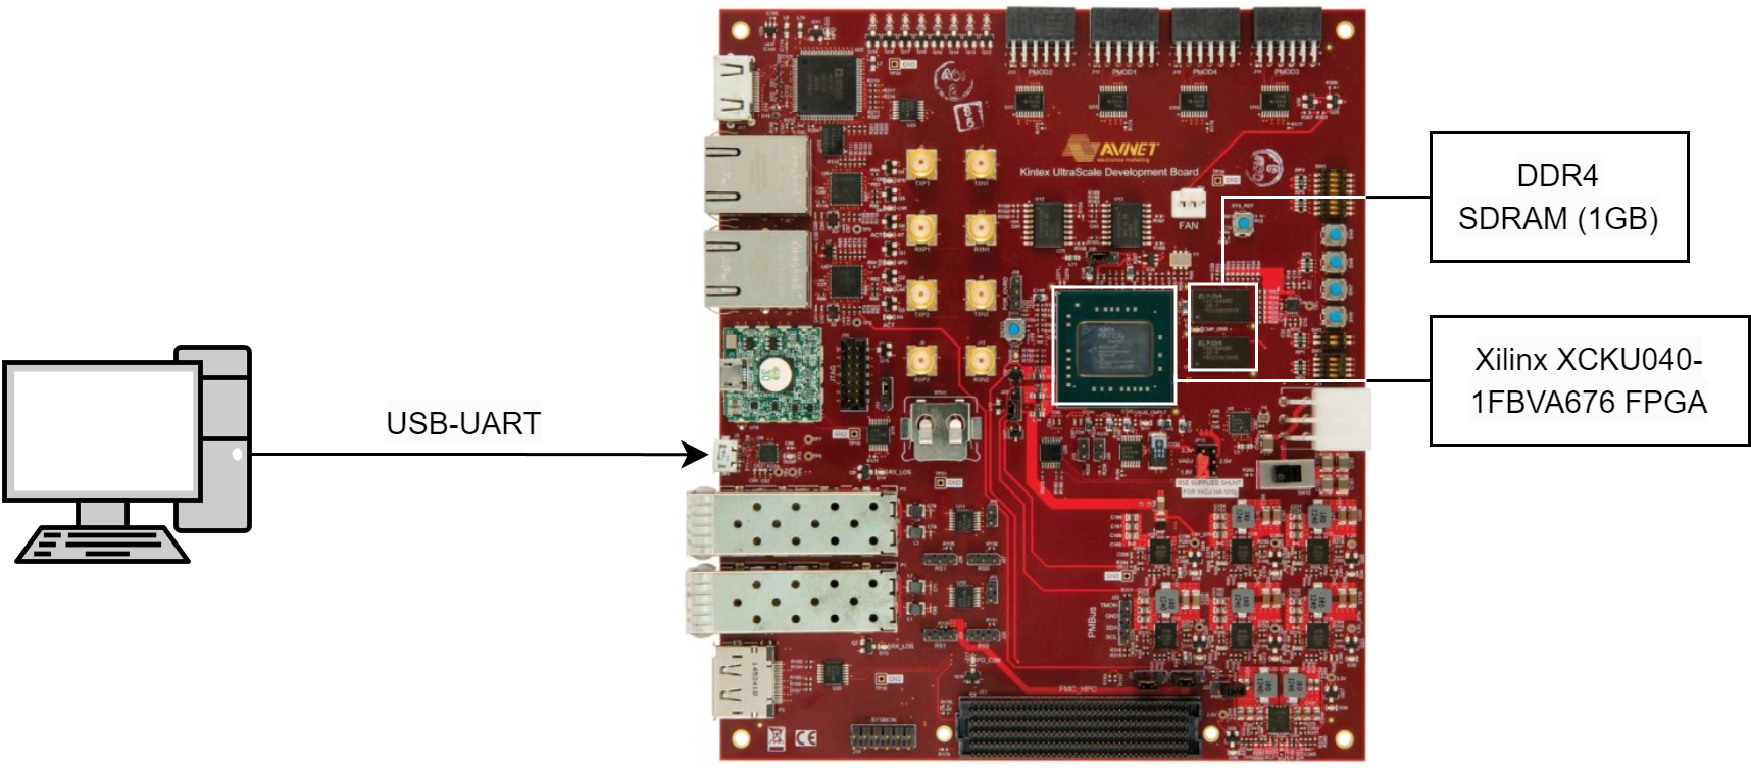
\includegraphics[width=0.80\linewidth]{system.pdf}}
\caption{Hardware setup overview.}
\label{system}
\end{figure}

The relevant components are the Xilinx XCKU040-1FBVA676 FPGA and the DDR4 SDRAM, as explained previously. Nonetheless, a basic description of how the hardware setup works is presented below.

\begin{itemize}
    \item \textbf{Personal Computer (PC):} The PC is responsible for the synthesis, compilation, and programming of IOb-MP2-E into the FPGA.
    \item \textbf{Xilinx Board:} The Xilinx board is an integral part of our hardware setup, housing the FPGA and related resources. This Xilinx board is where IOb-MP2-E is ultimately implemented and executed.
    \item \textbf{USB-UART Connection:} To facilitate communication between the PC and the Xilinx board, a USB-UART connection is employed. This connection is utilized for transferring the synthesized configuration bitstream from the PC to the FPGA.
    \item \textbf{Compilation and Synthesis Software:} On the PC, specialized compilation and synthesis software tools are used to design and compile IOb-MP2-E. These tools generate a configuration bitstream that specifies the functionality and behavior of IOb-MP2-E. Once generated, this bitstream is transferred to the Xilinx board via the USB connection.
    \item \textbf{FPGA Implementation:} The FPGA is responsible for the physical implementation of IOb-MP2-E.
    \item \textbf{IOb-MP2-E Execution:} Once the IOb-MP2-E is successfully implemented in the FPGA, it can be executed within the FPGA's logic fabric. The SoC interacts with other components on the Xilinx board, such as DDR memory, to carry out the intended computational tasks.
\end{itemize}

